\clearpage



\appendix

\section{Regression figures}\label{app:regression}

\begin{figure}[h!]
    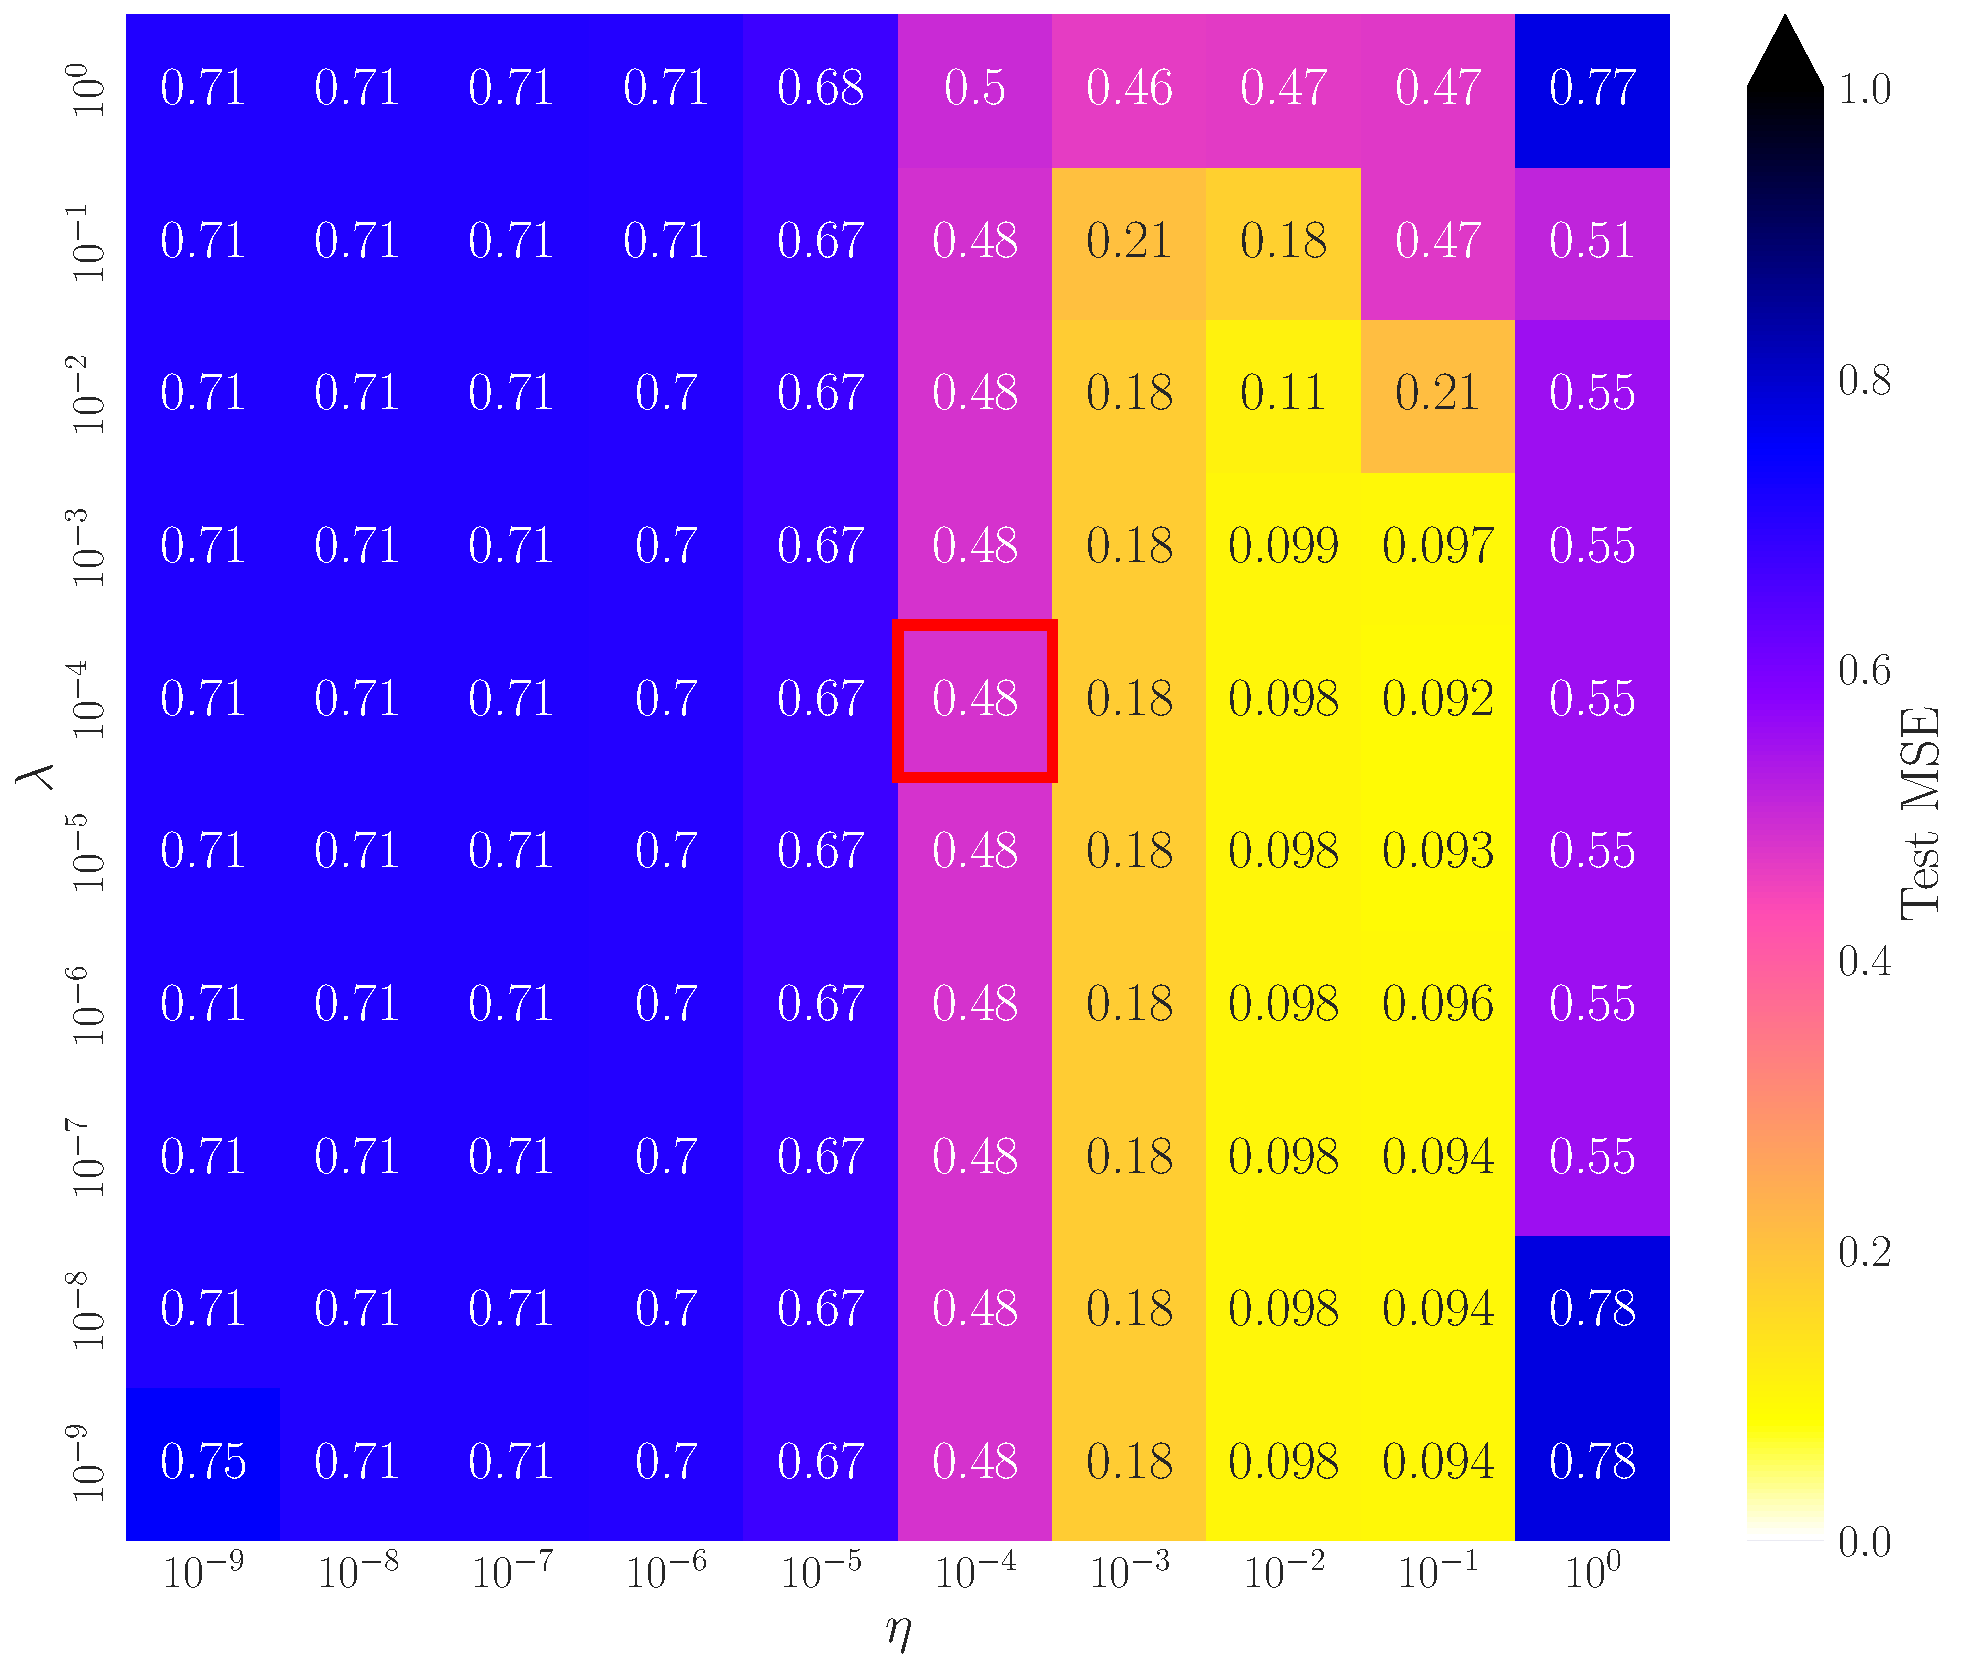
\includegraphics[width=\linewidth]{eta_lambda_analysis.pdf}
    \caption{Heatmap of the MSE as function of learning rate $\eta$ and regularisation parameter $\lambda$, using SGD with RMSProp as optimiser performing regression analysis of a 3 layered, 15-10-5 neurons, neural network. }
    \label{fig:reg_eta_lambda}
\end{figure}

\begin{figure}[h!]
    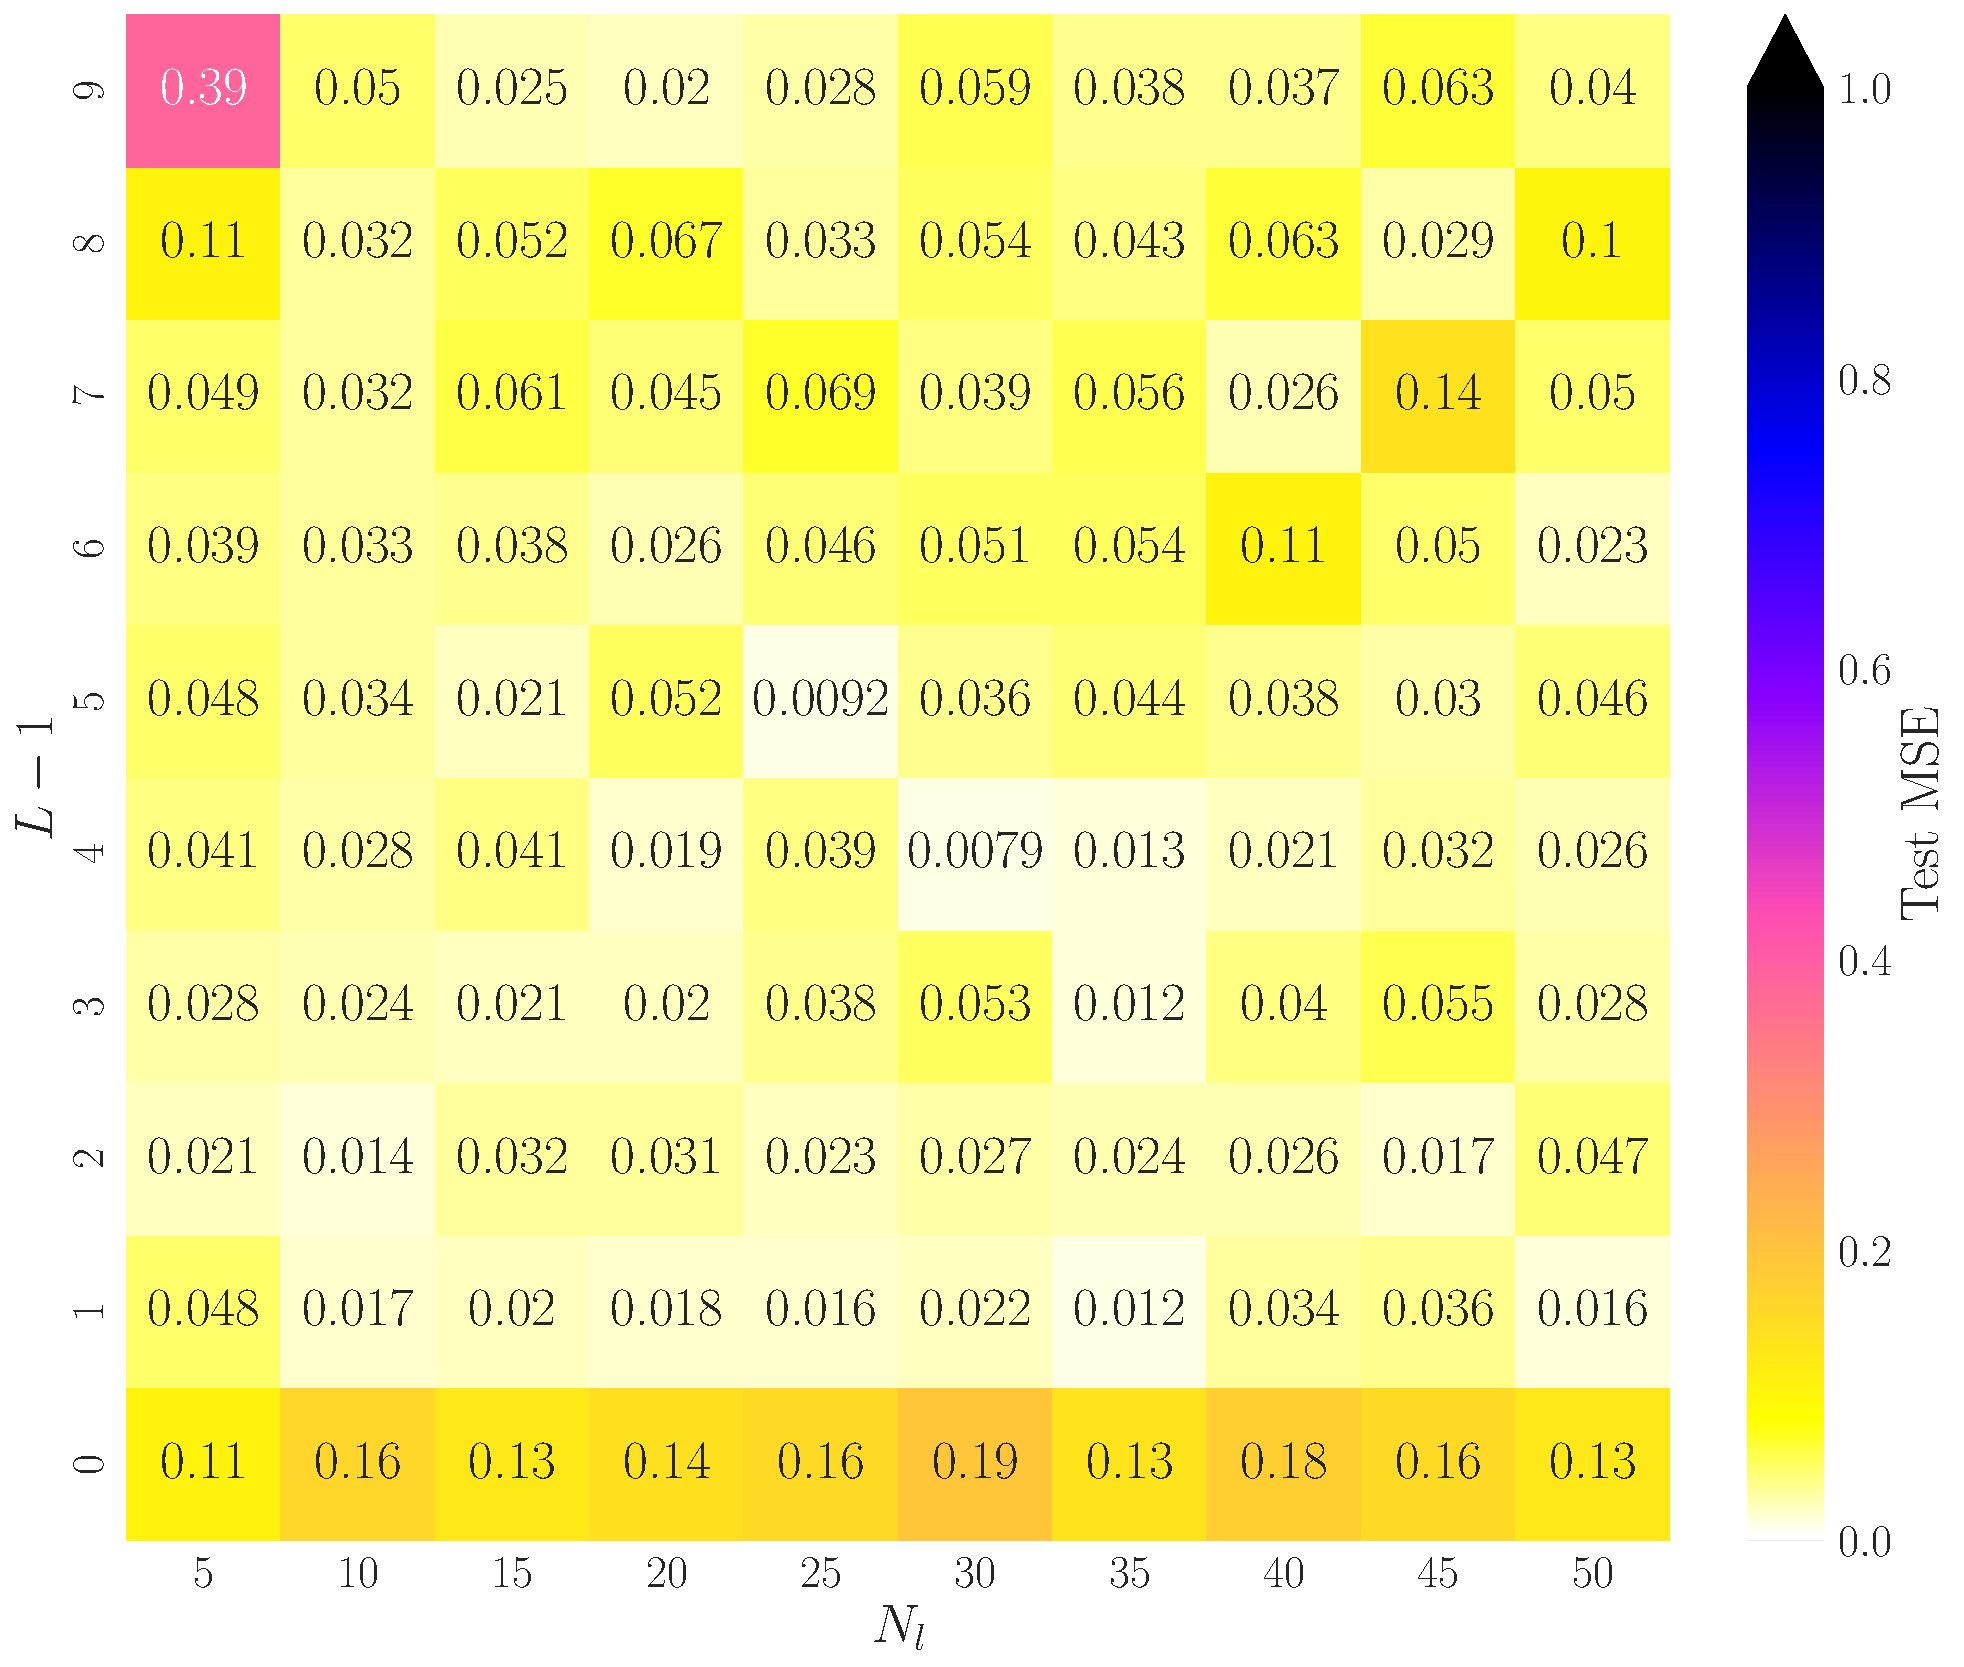
\includegraphics[width=\linewidth]{layer_neuron_analysis.pdf}
    \caption{Heatmap of the MSE as function of hidden layers $L-1$ and neurons per layer $N_l$, using SGD with RMSProp as optimiser performing regression analysis with $\eta=10^{-1}$ and $\lambda=10^{-4}$.}
    \label{fig:reg_layer_neuron}
\end{figure}

\begin{figure}[h!]
    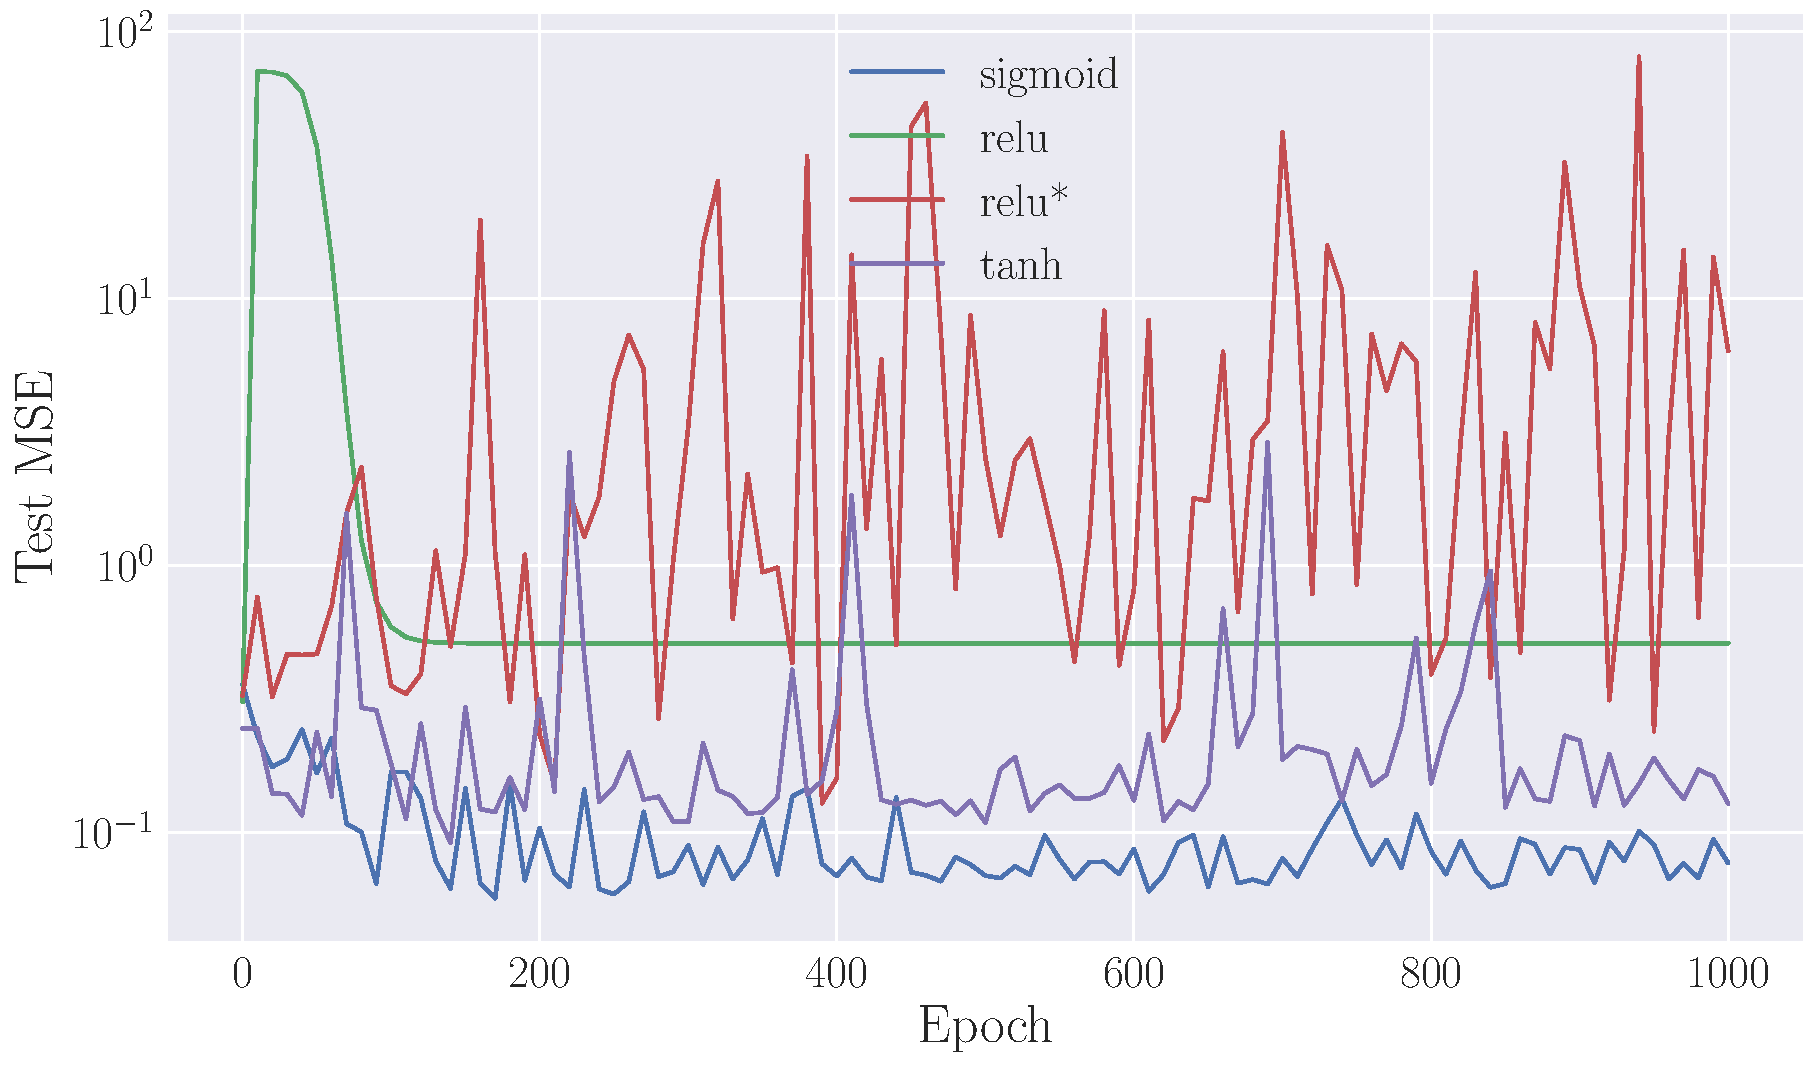
\includegraphics[width=\linewidth]{actFuncPer1000Epoch.pdf}
    \caption{Plot of the MSE for up to 1000 epochs, using SGD with RMSProp as optimiser performing regression analysis with $L-1=1$ hidden layer with $N_l=30$ neurons with $\eta=10^{-1}$ and $\lambda=10^{-4}$. The four different activation functions perform differently. Note the logarithmic MSE axis.}
    \label{fig:reg_act_epoch1000}
\end{figure}

\begin{figure}[h!]
    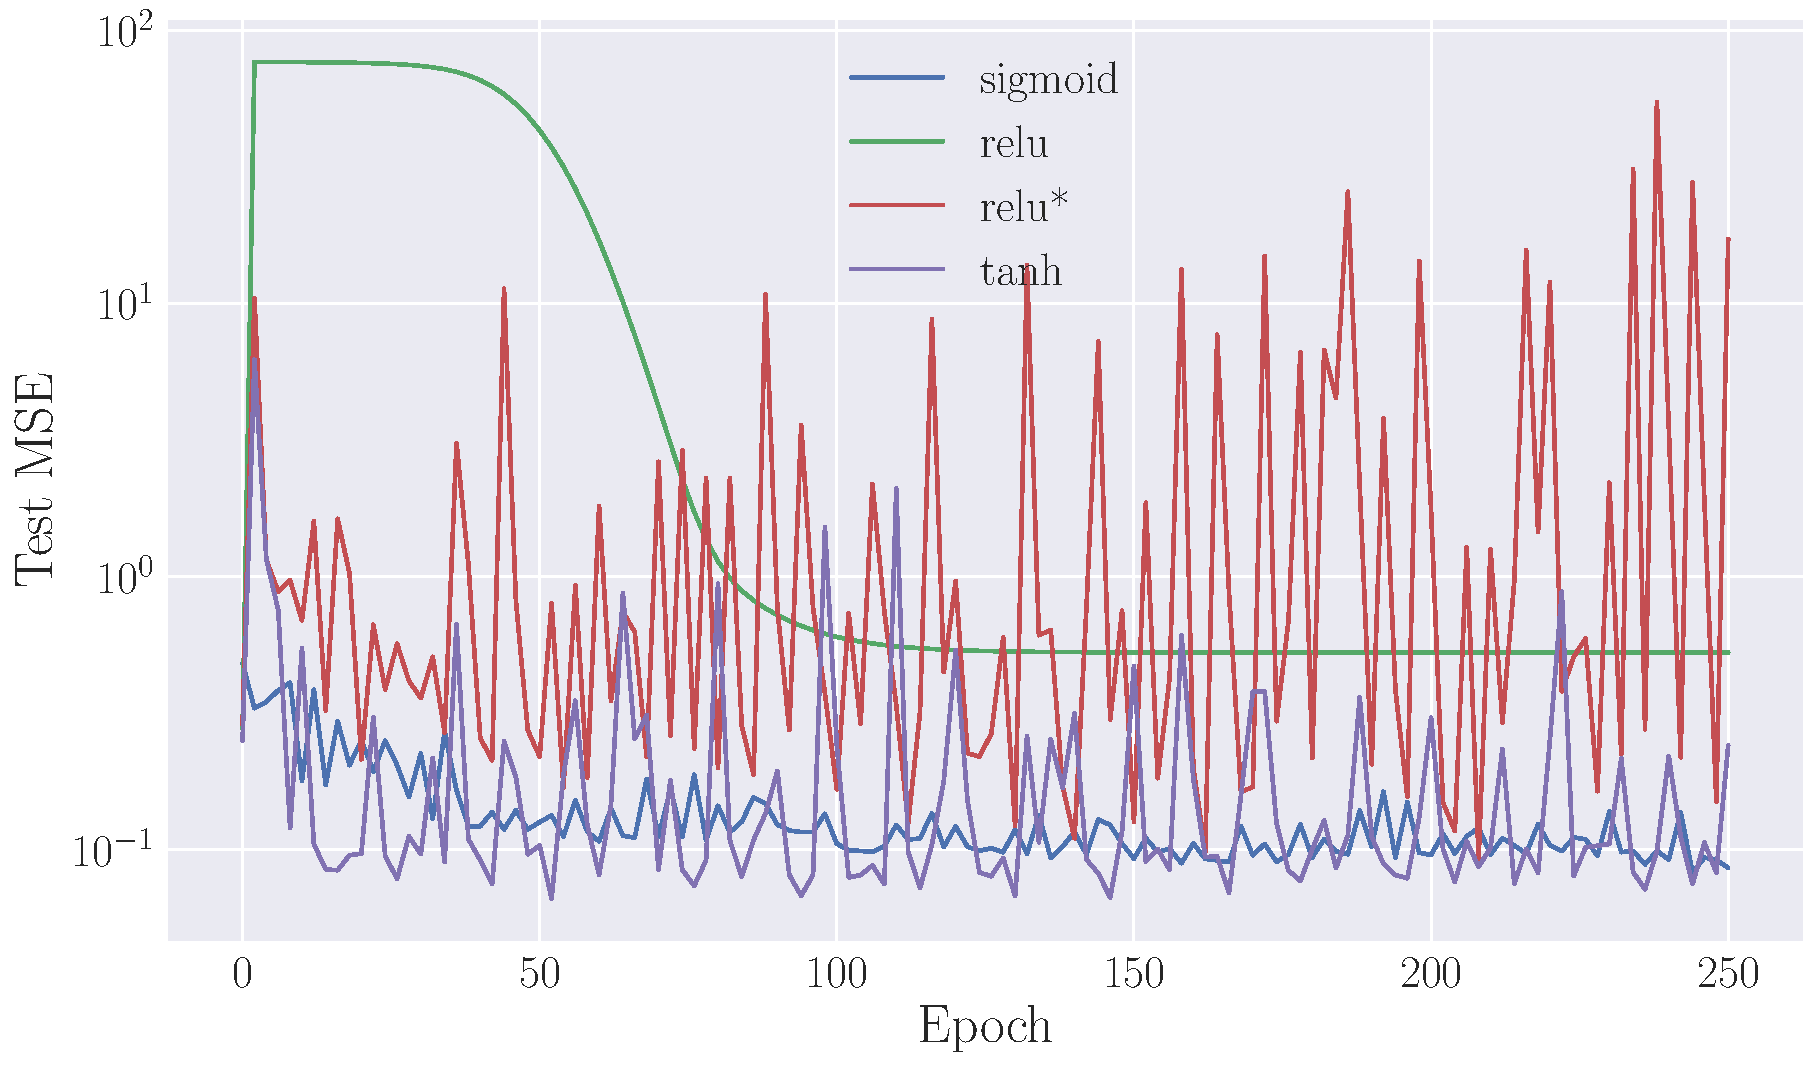
\includegraphics[width=\linewidth]{actFuncPerEpoch.pdf}
    \caption{Plot of the MSE for up to 250 epochs, using SGD with RMSProp as optimiser performing regression analysis with $L-1=1$ hidden layer with $N_l=30$ neurons with $\eta=10^{-1}$ and $\lambda=10^{-4}$. The four different activation functions perform differently. Note the logarithmic MSE axis.}
    \label{fig:reg_act_epoch}
\end{figure}

\begin{figure}[h!]
    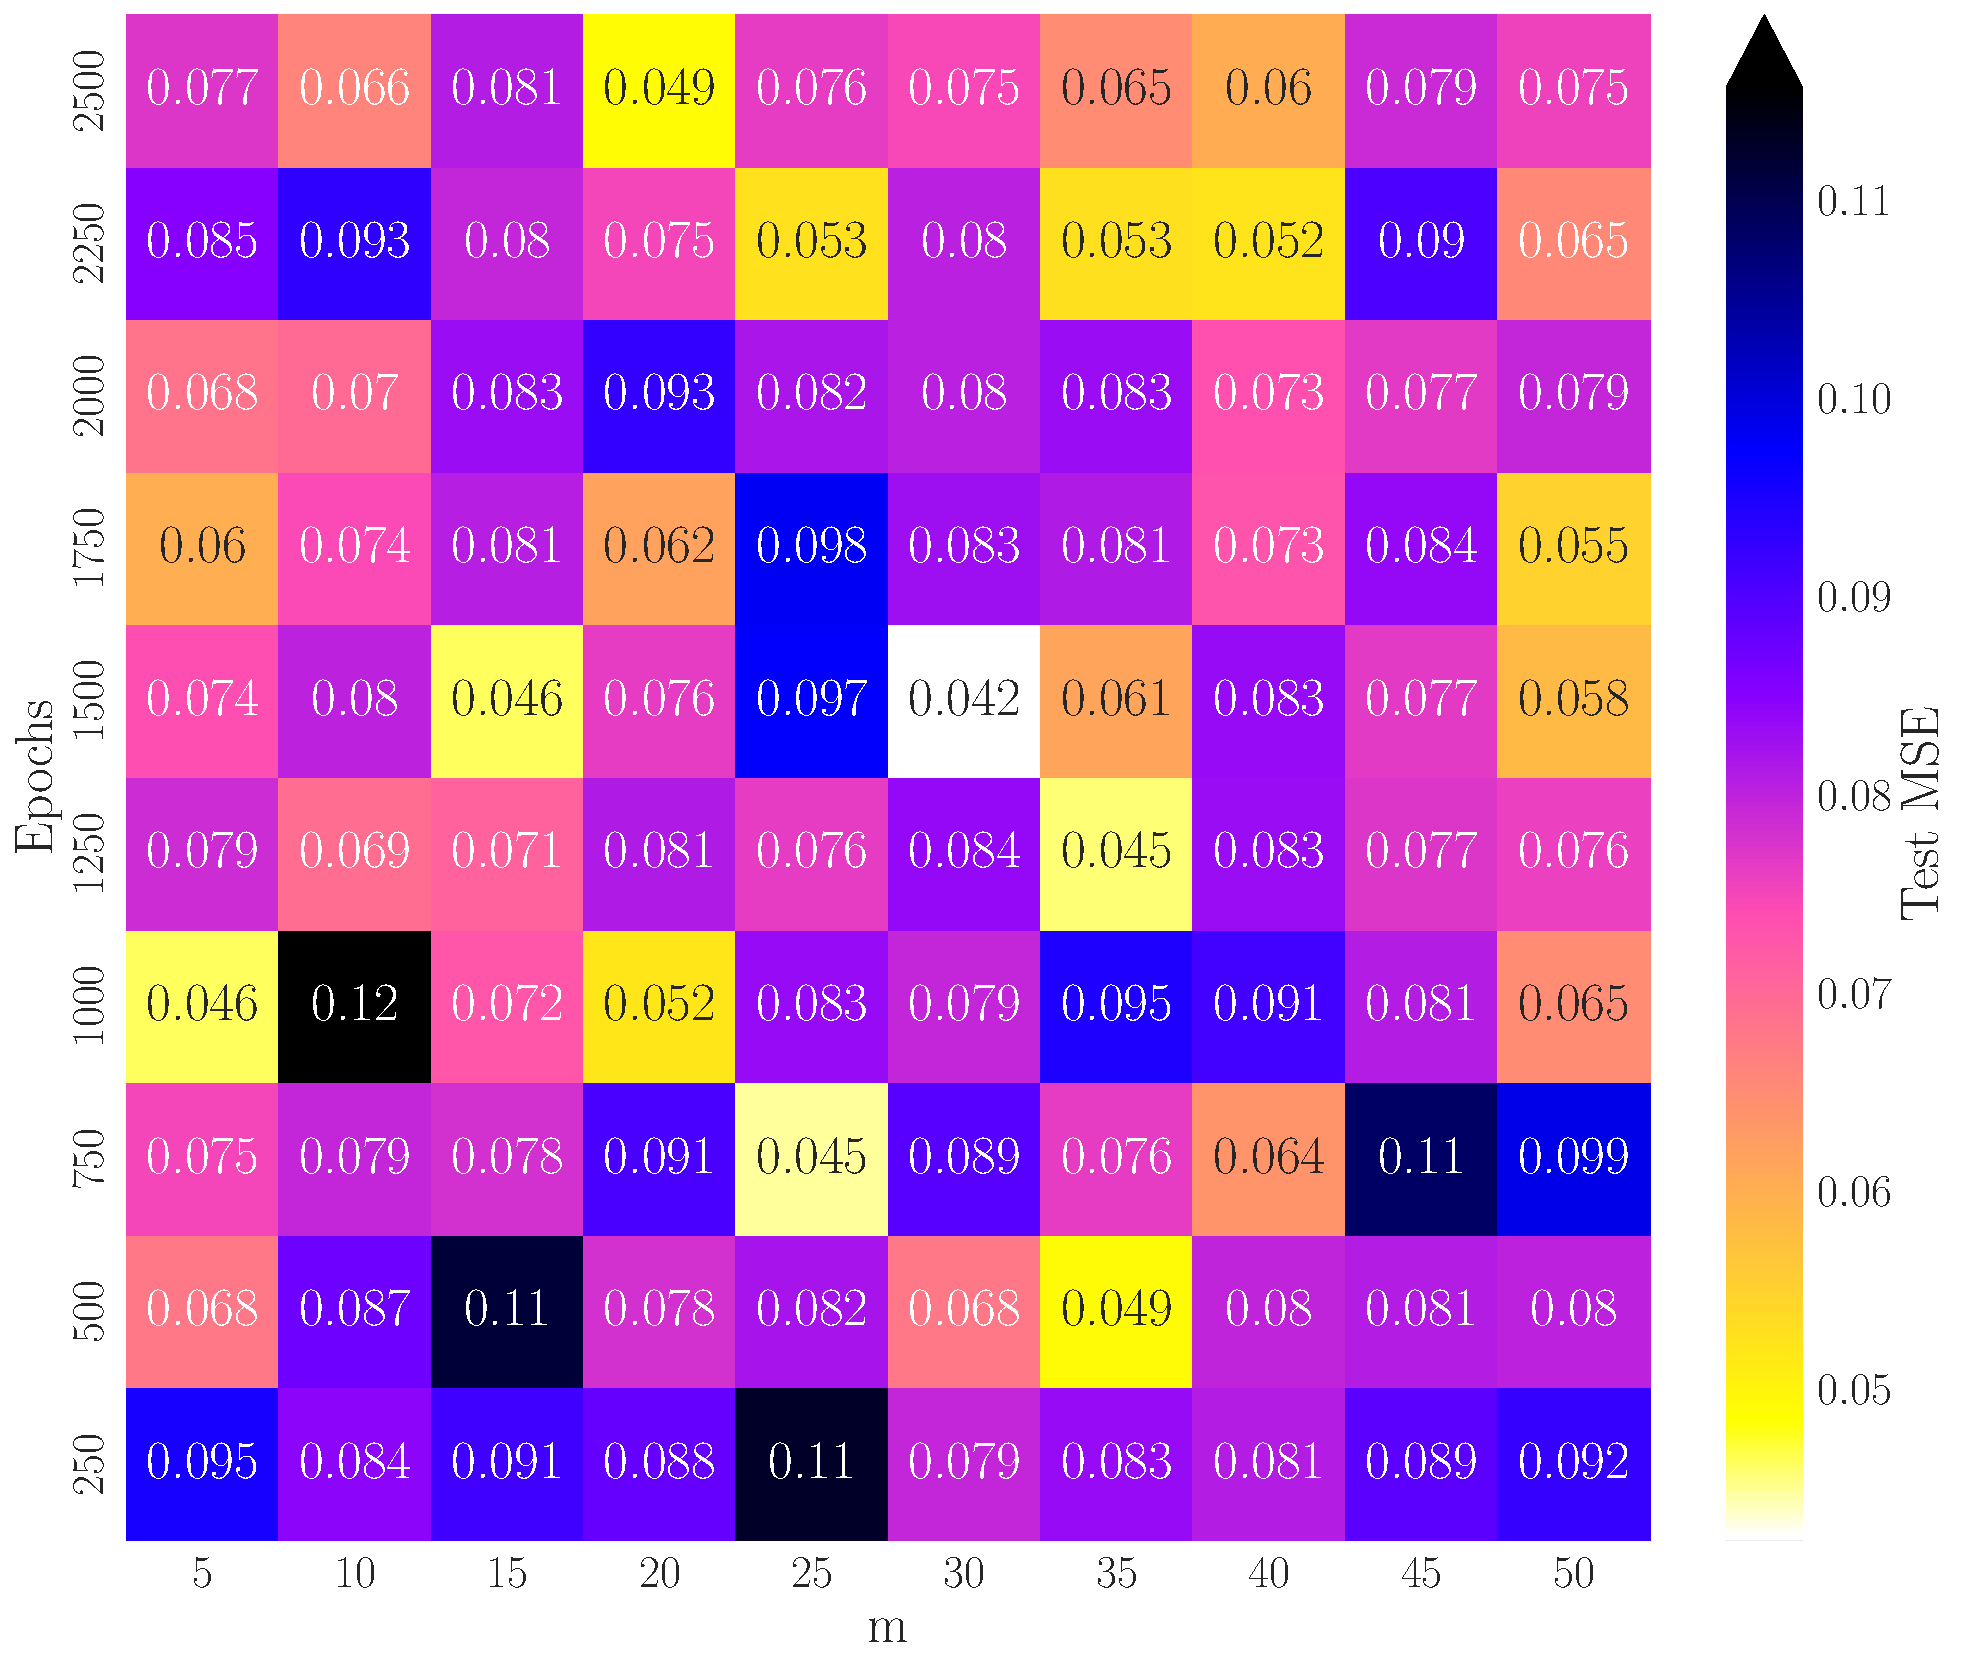
\includegraphics[width=\linewidth]{epoch_minibatch_analysis.pdf}
    \caption{Heatmap of the MSE as function of the number of minibatches $m$ and training epochs, using SGD with RMSProp as optimiser performing regression analysis with $L-1=1$ hidden layer with $N_l=30$ neurons with $\eta=10^{-1}$ and $\lambda=10^{-4}$ using sigmoid as activation function. }
    \label{fig:reg_minibatch_epoch}
\end{figure}




\clearpage

\section{Classification figures}\label{app:classification}

\begin{figure}[h!]
    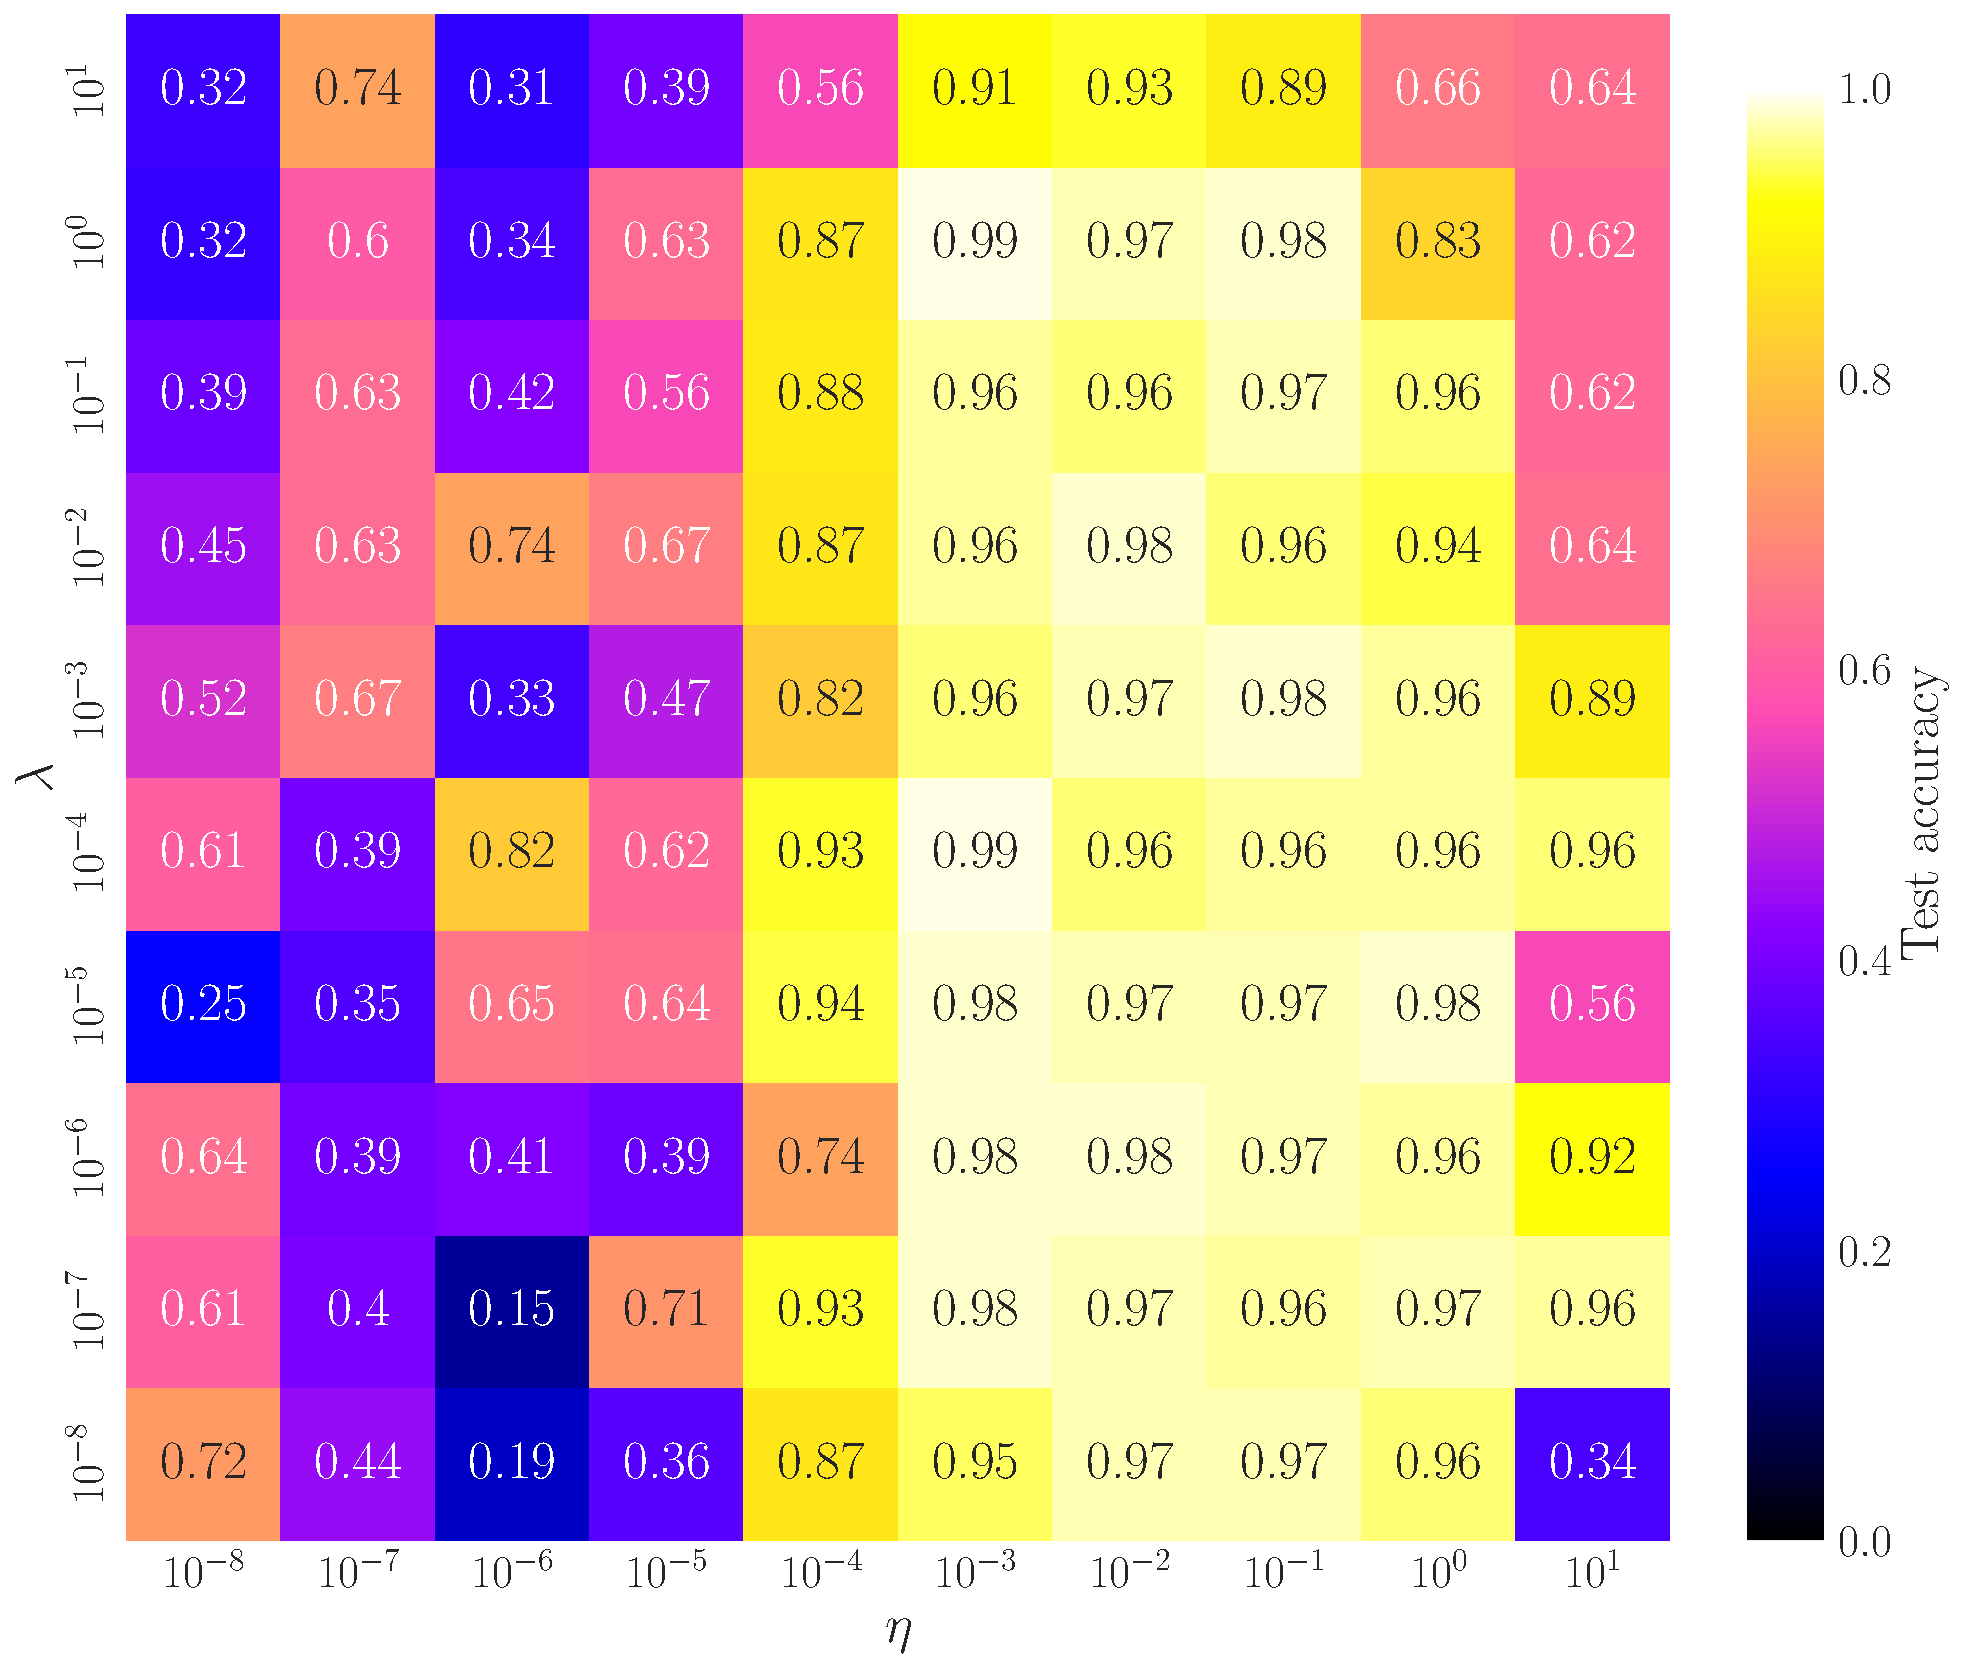
\includegraphics[width=\linewidth]{eta_lambda_analysisCancer.pdf}
    \caption{Heatmap of accuracy as function of learning rate $\eta$ and regularisation parameter $\lambda$, using SGD with RMSProp as optimiser performing regression analysis of a 3 layered, 15-10-5 neurons, neural network. }
    \label{fig:class_eta_lambda}
\end{figure}

\begin{figure}[h!]
    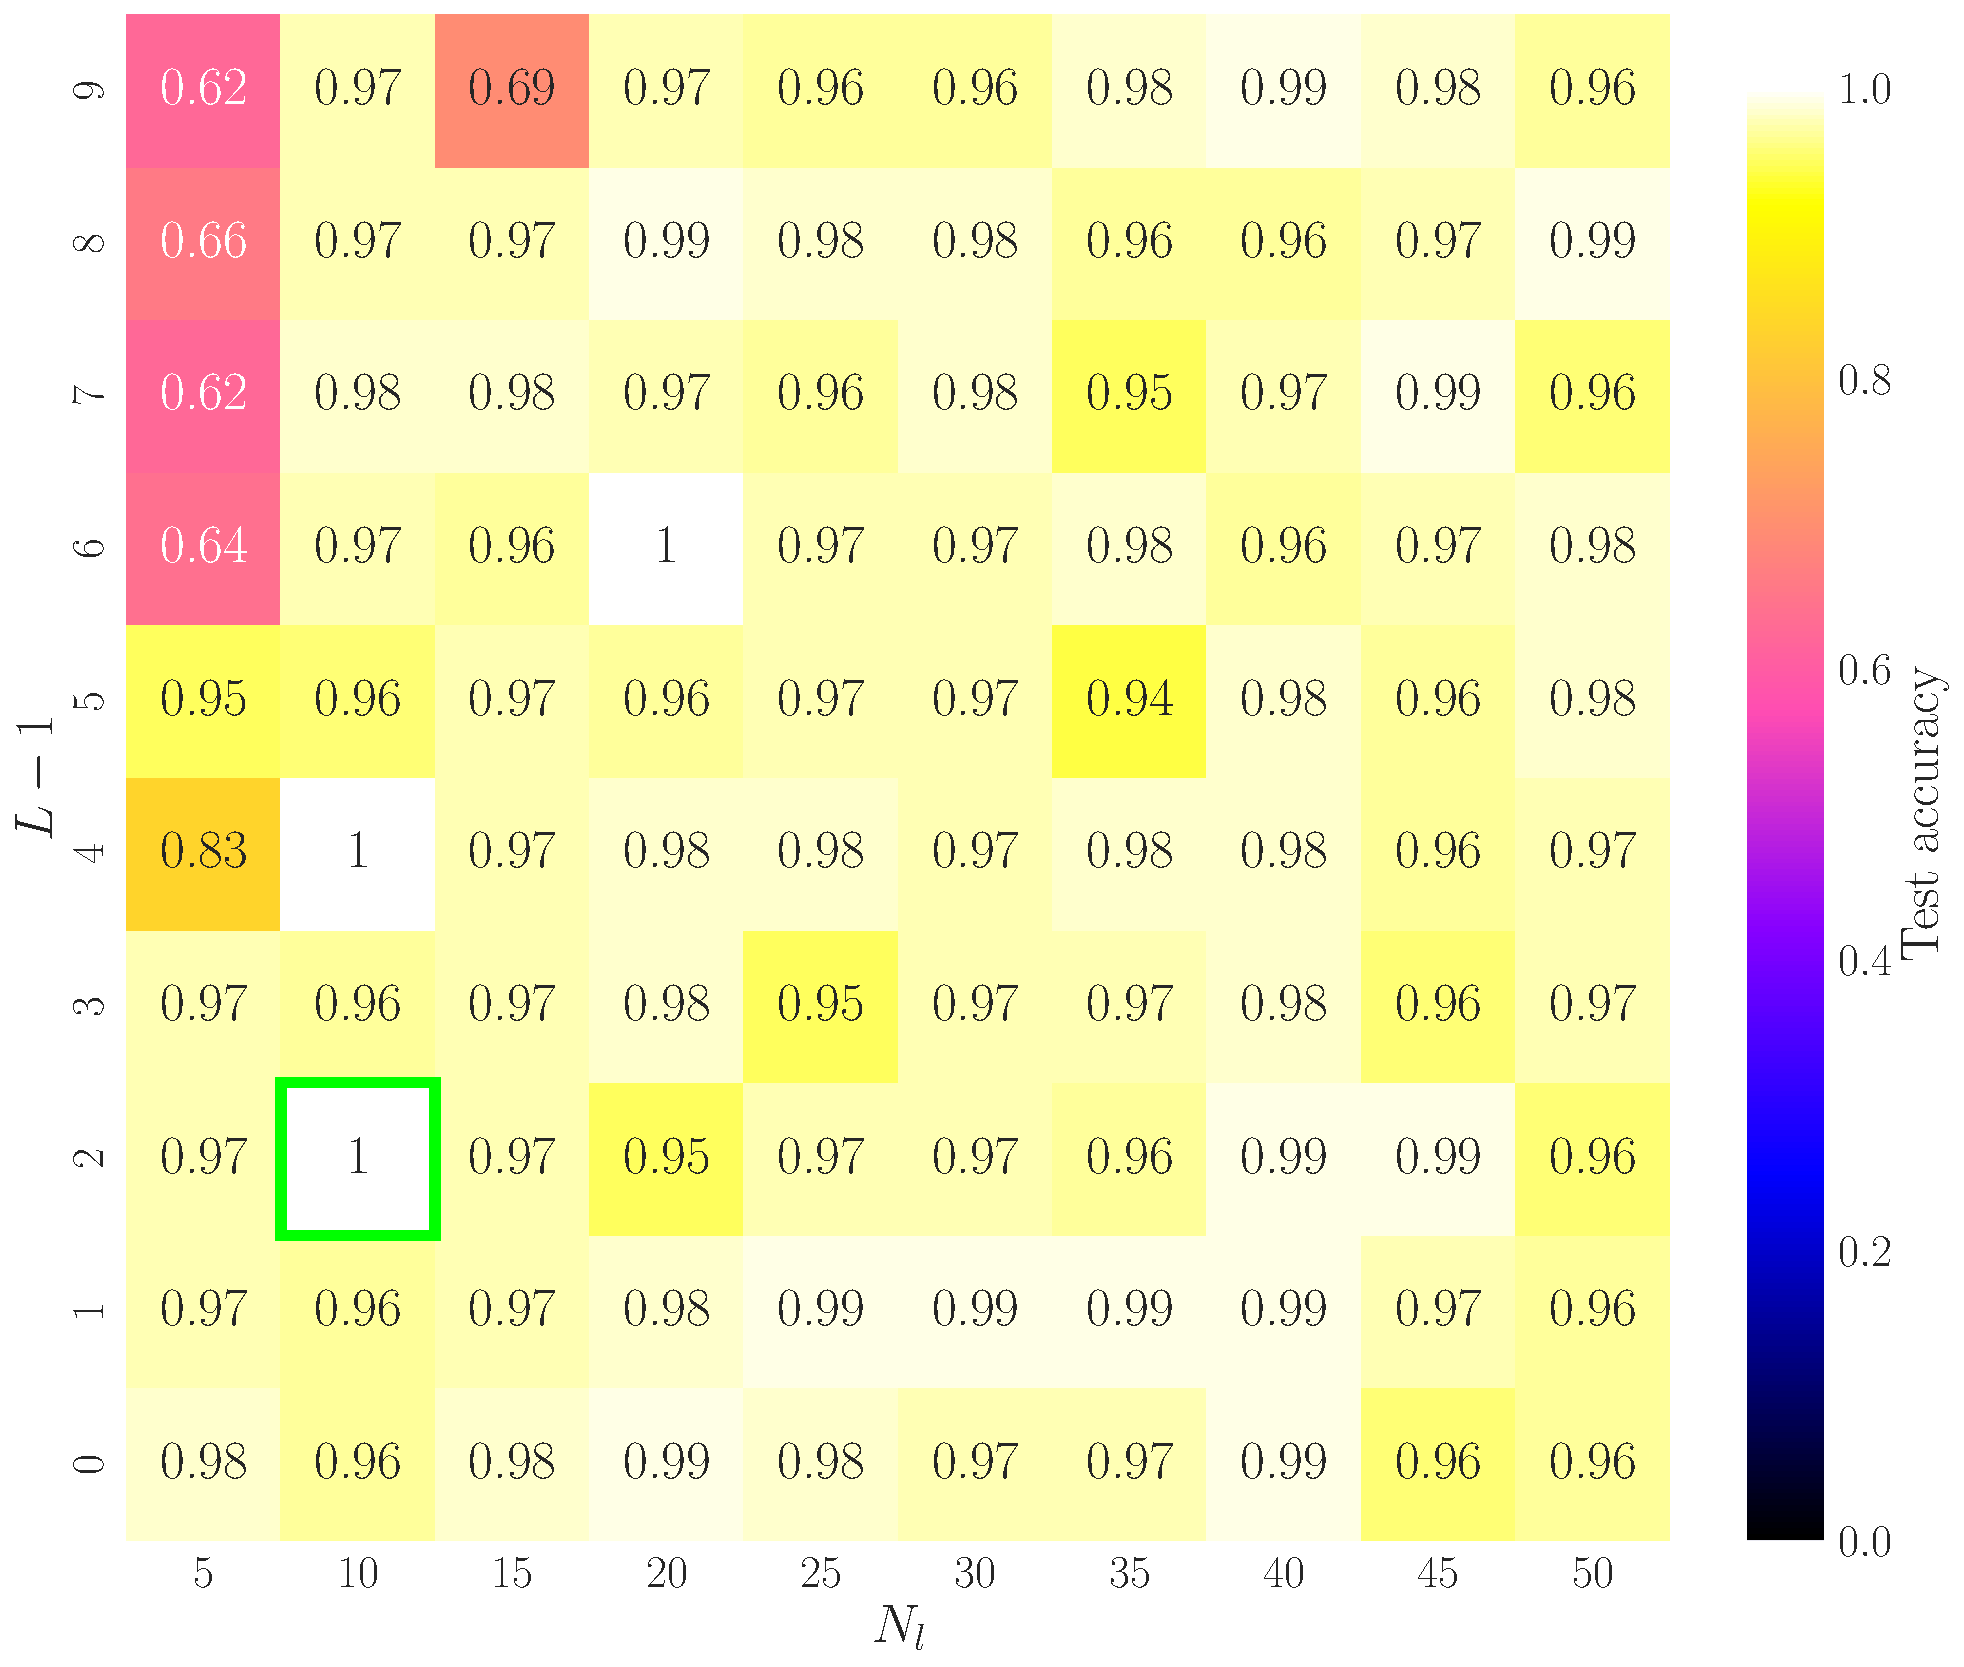
\includegraphics[width=\linewidth]{layer_neuron_analysisCancer.pdf}
    \caption{Heatmap of accuracy as function of hidden layers $L-1$ and neurons per layer $N_l$, using SGD with RMSProp as optimiser performing regression analysis with $\eta=10^{-3}$ and $\lambda=10^{-6}$.}
    \label{fig:class_layer_neuron}
\end{figure}

\begin{figure}[h!]
    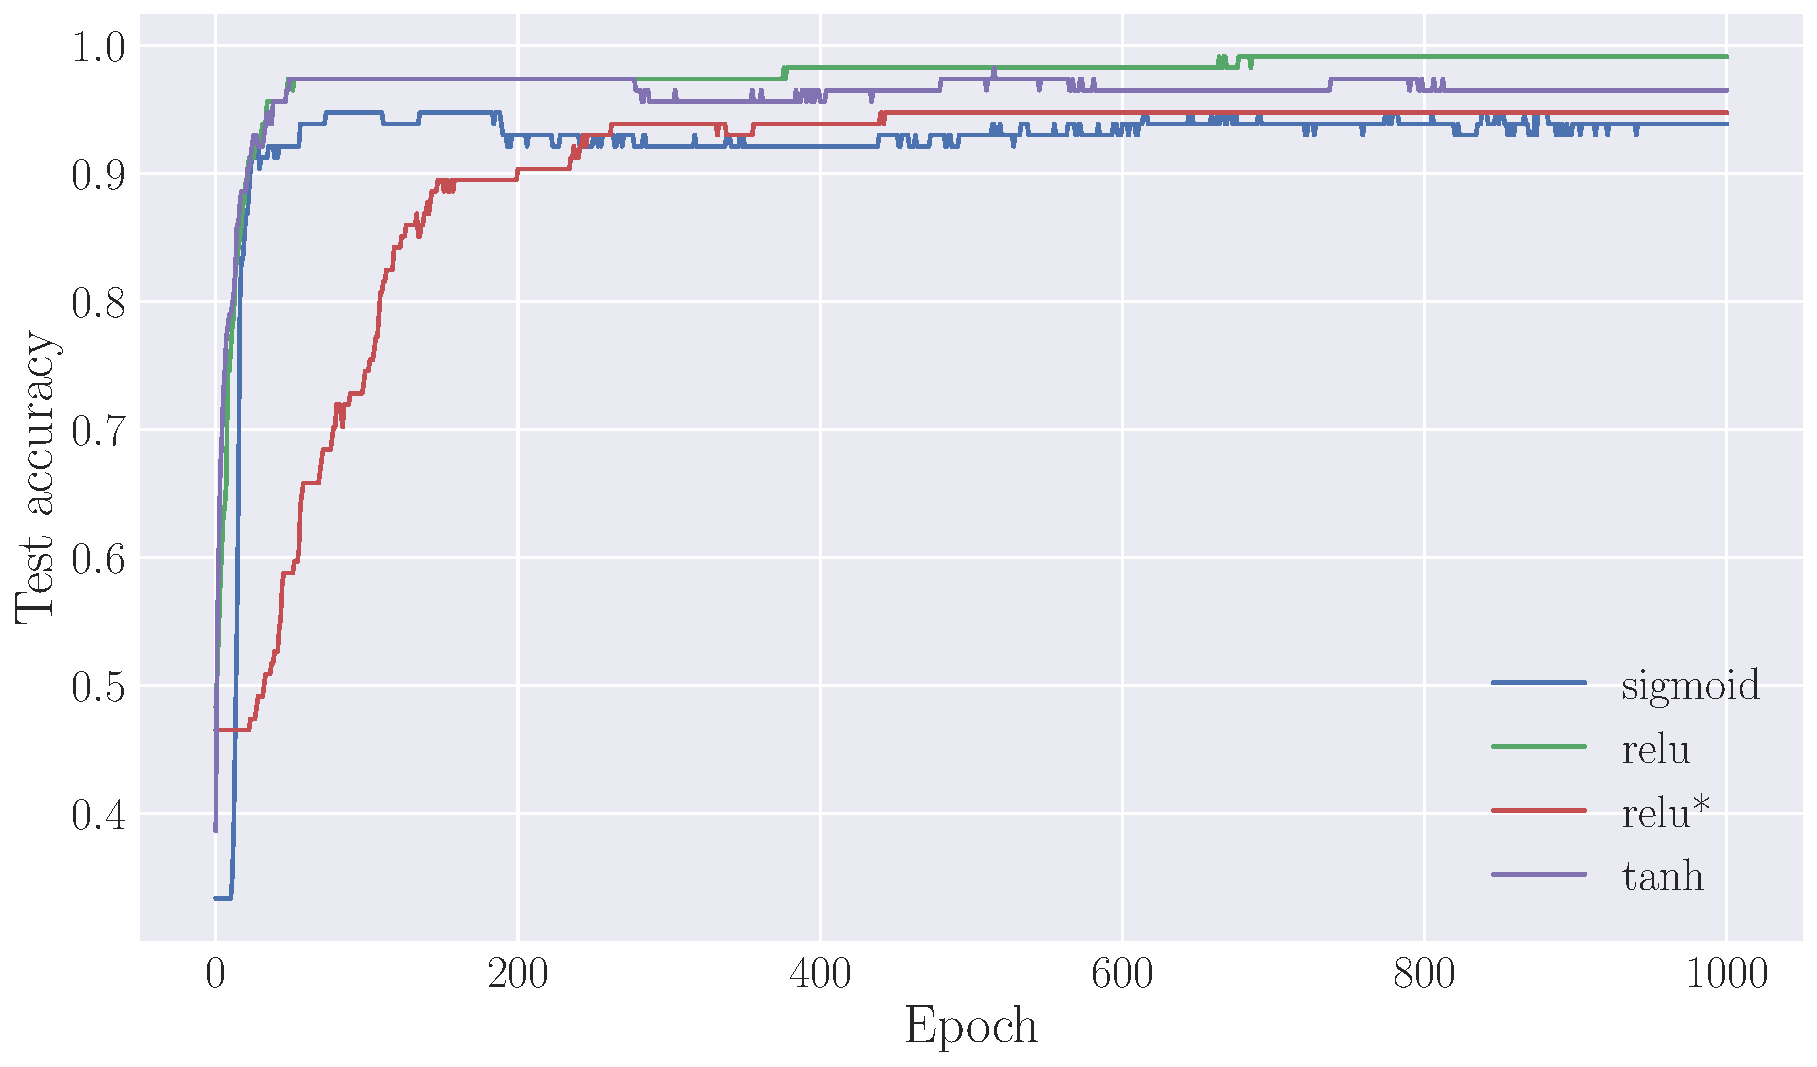
\includegraphics[width=\linewidth]{actFuncPerEpoch1000Cancer.pdf}
    \caption{Plot of accuracy for up to 1000 epochs, using SGD with RMSProp as optimiser performing regression analysis with $L-1=2$ hidden layers with $N_l=10$ neurons each with $\eta=10^{-3}$ and $\lambda=10^{-6}$. The four different activation functions perform differently.}
    \label{fig:class_act_epoch1000}
\end{figure}

\begin{figure}[h!]
    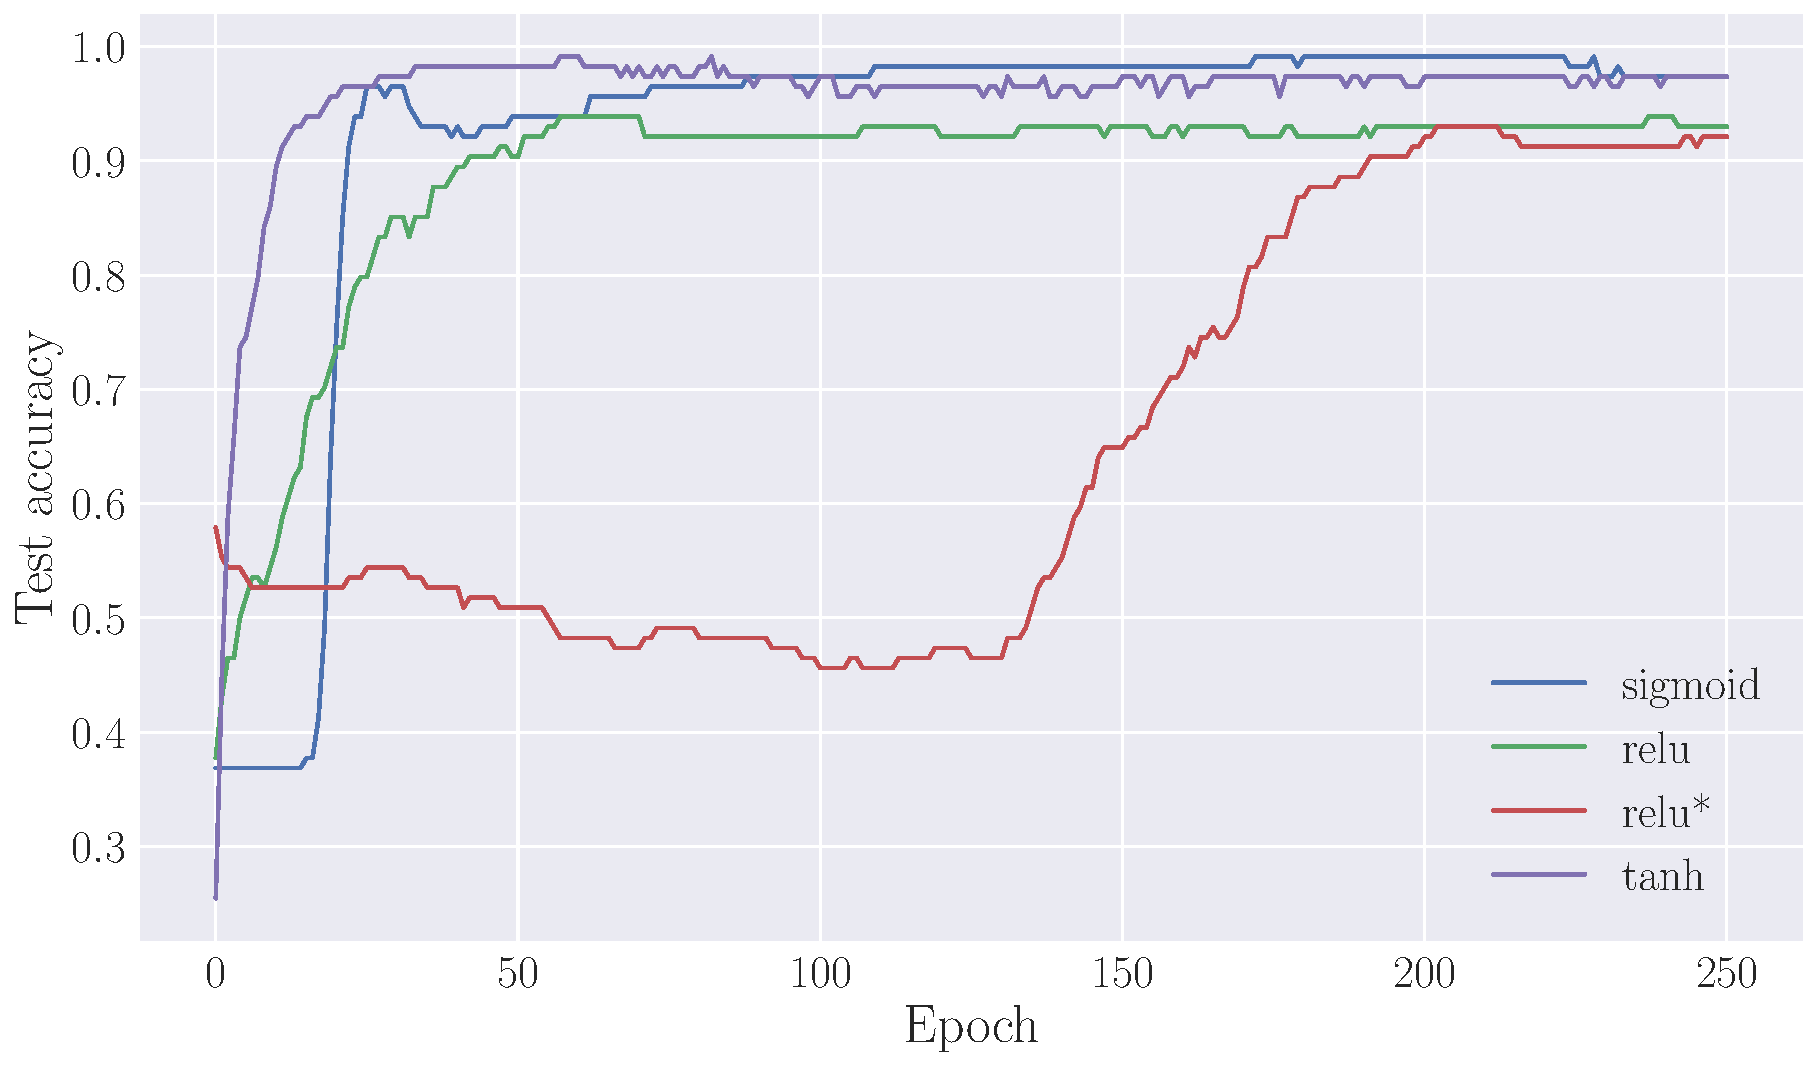
\includegraphics[width=\linewidth]{actFuncPerEpochCancer.pdf}
    \caption{Plot of accuracy for up to 250 epochs, using SGD with RMSProp as optimiser performing regression analysis with $L-1=2$ hidden layer with $N_l=10$ neurons with $\eta=10^{-3}$ and $\lambda=10^{-6}$. The four different activation functions perform differently.}
    \label{fig:class_act_epoch}
\end{figure}

\begin{figure}[h!]
    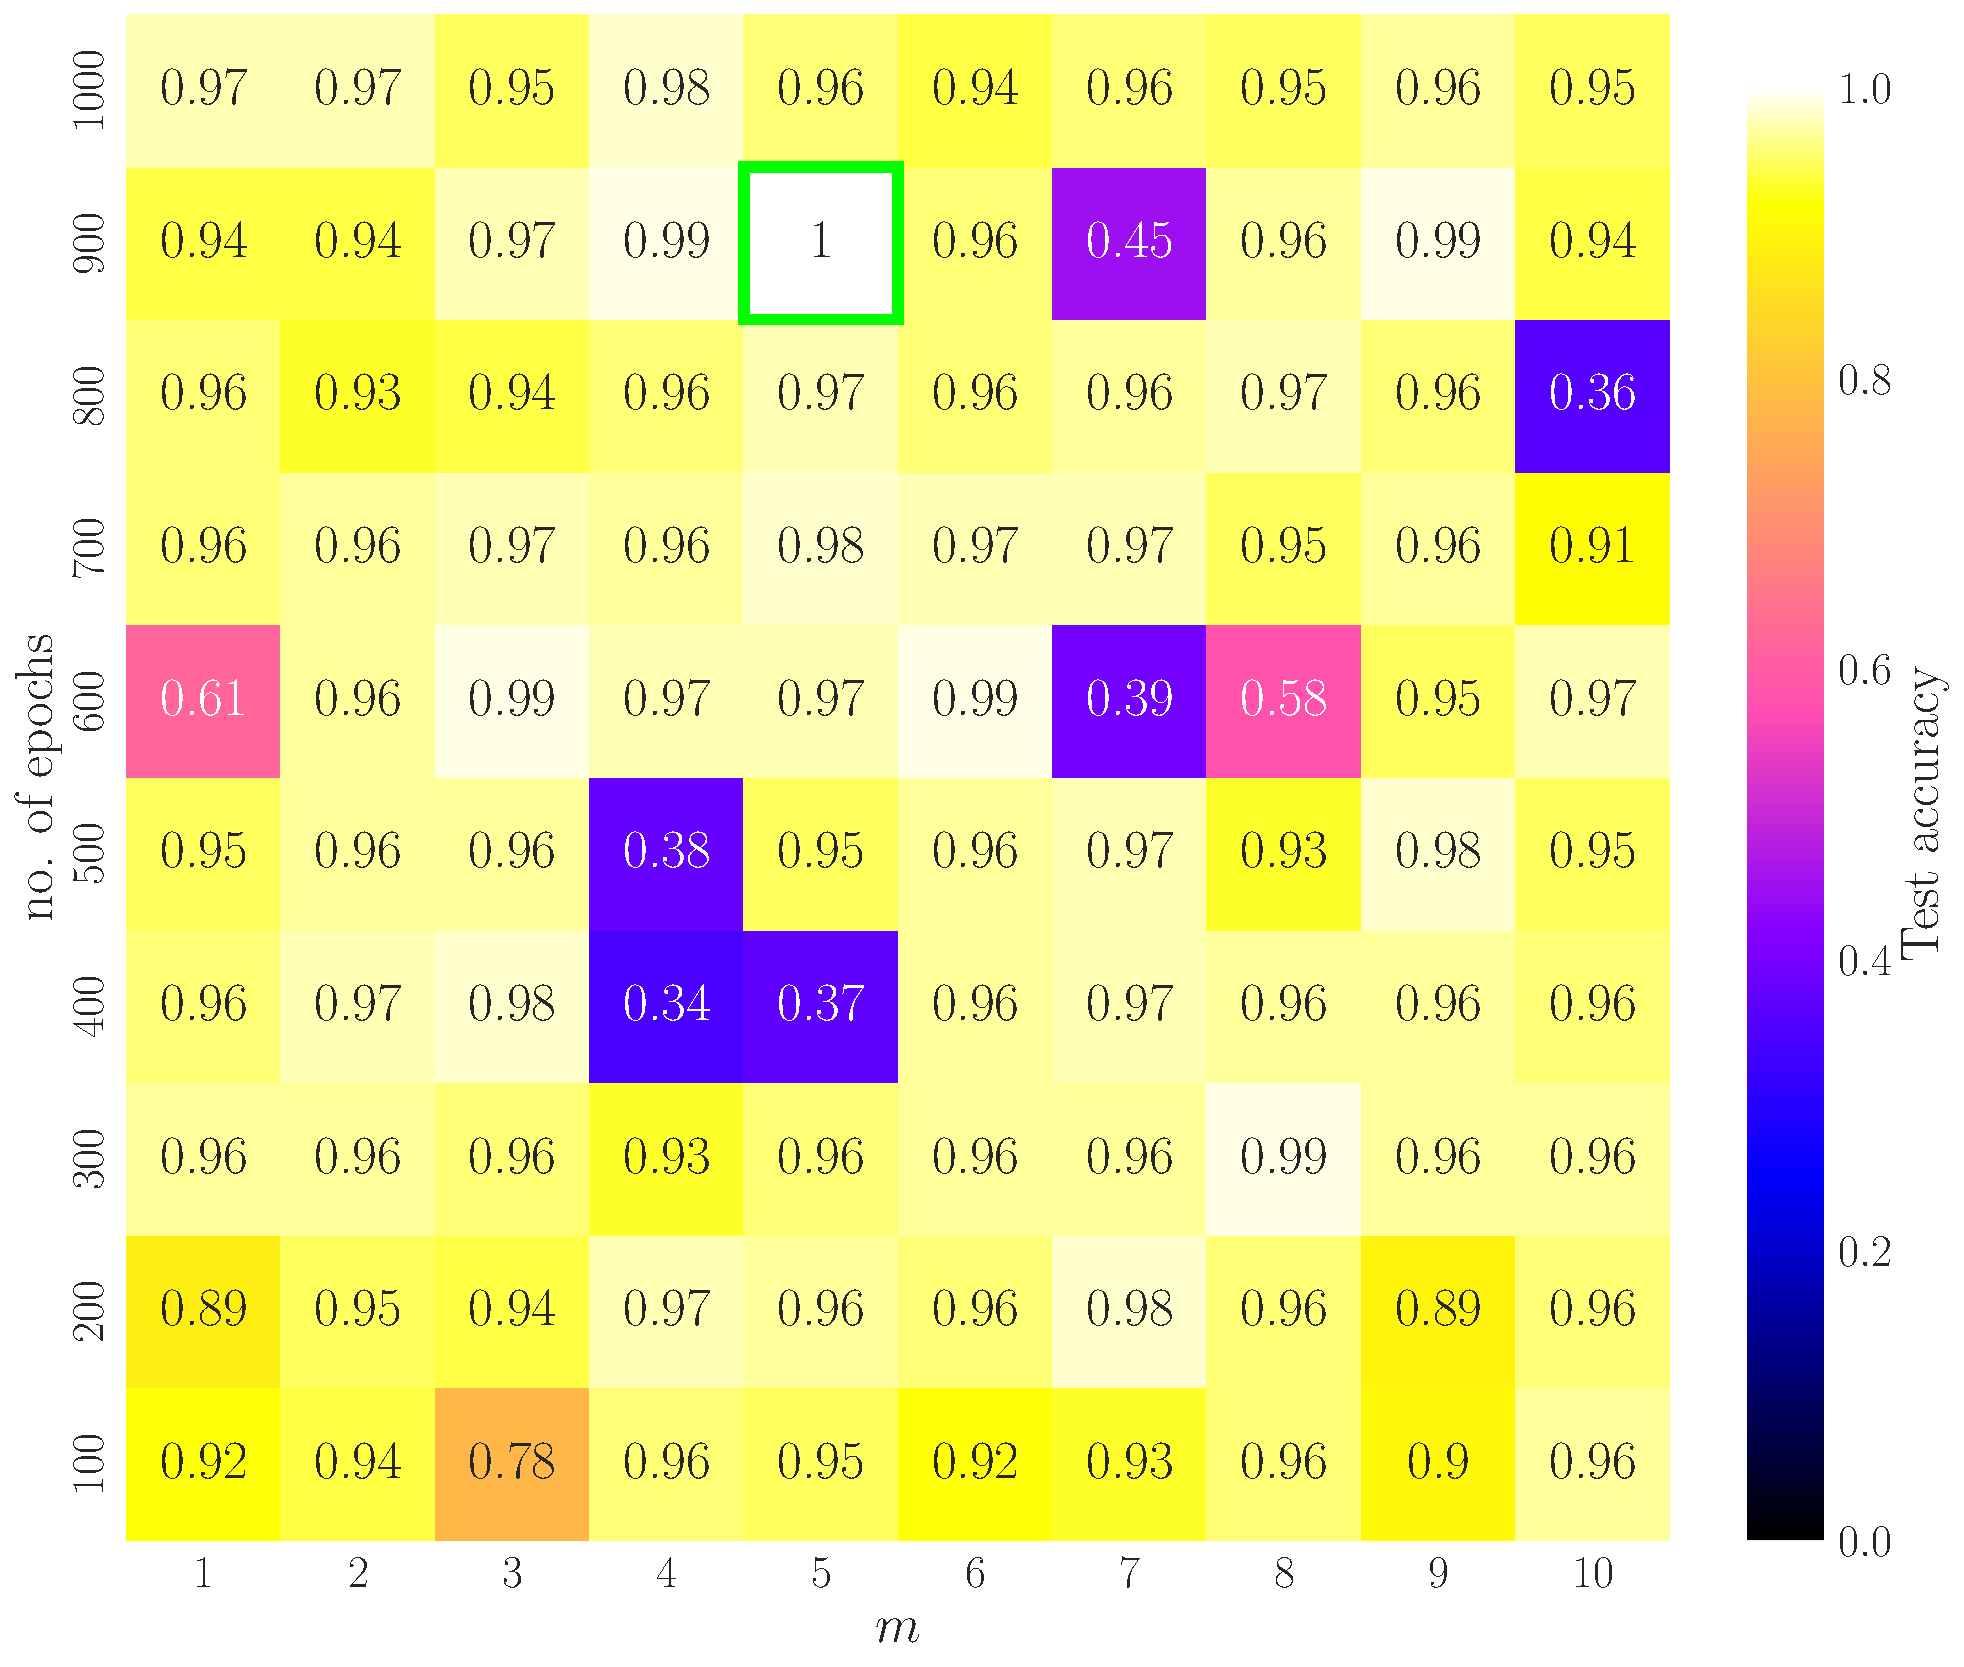
\includegraphics[width=\linewidth]{epoch_minibatch_analysisCancer.pdf}
    \caption{Heatmap of accuracy as function of the number of minibatches $m$ and training epochs, using SGD with RMSProp as optimiser performing regression analysis with $L-1=2$ hidden layer with $N_l=10$ neurons with $\eta=10^{-3}$ and $\lambda=10^{-6}$ using RELU as activation function. }
    \label{fig:class_minibatch_epoch}
\end{figure}


\clearpage

\section{Logistic regression figure}\label{app:logistic}

\begin{figure}[h!]
    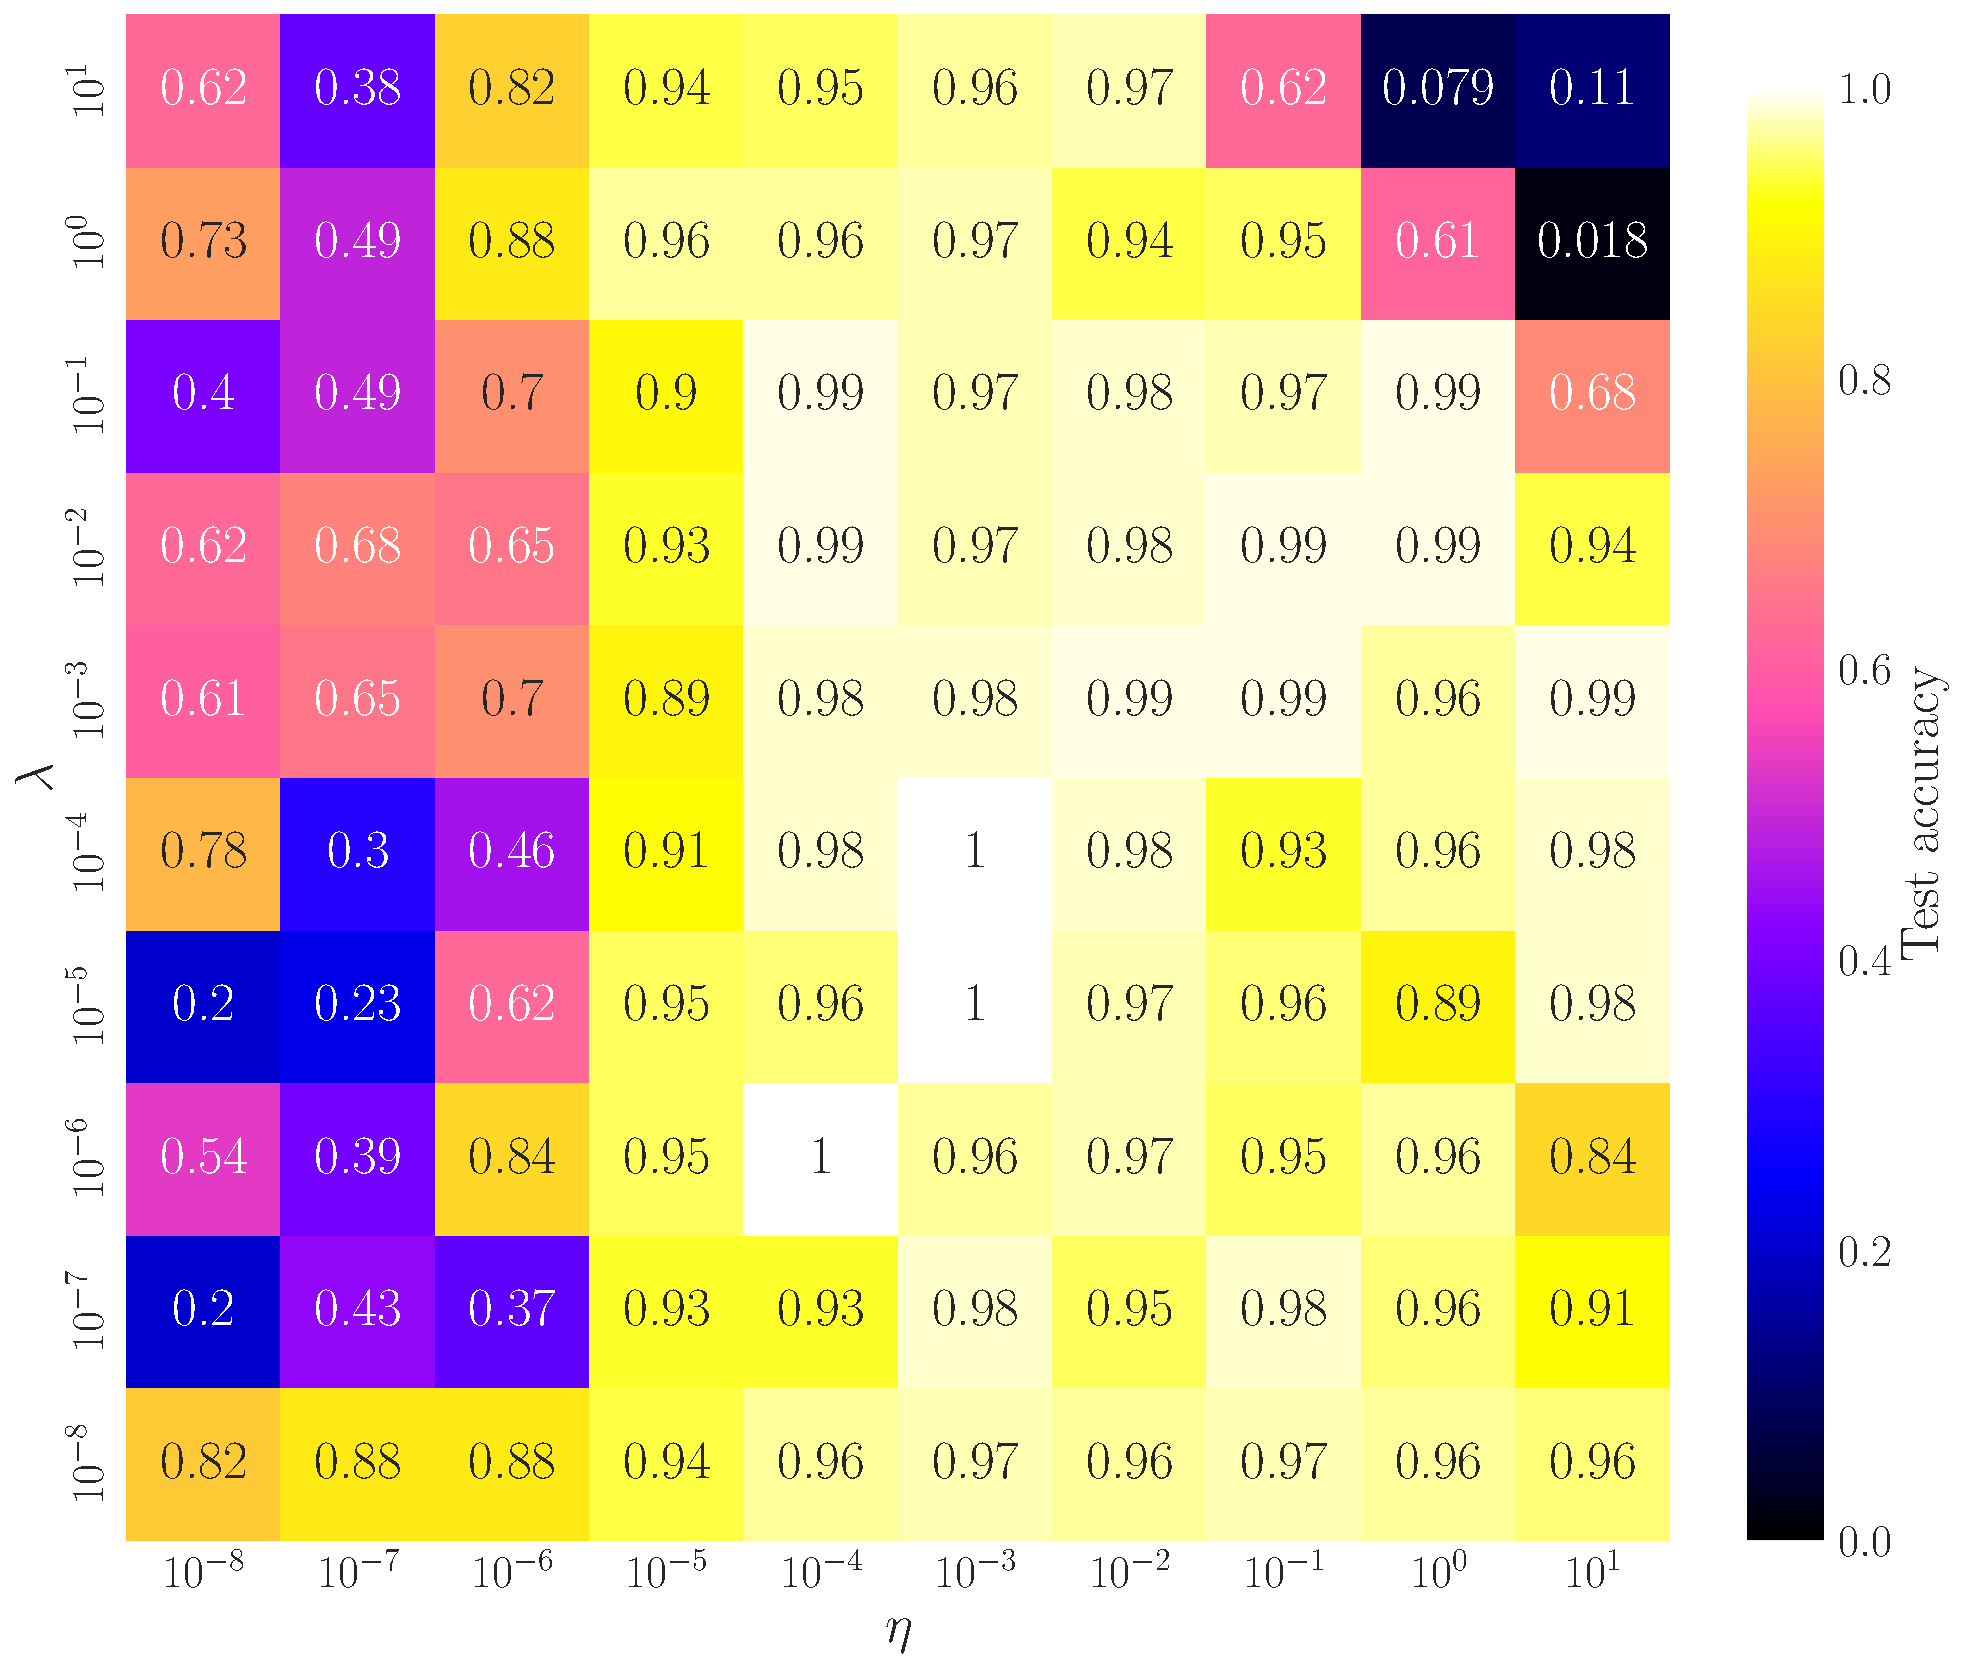
\includegraphics[width=\linewidth]{logistic.pdf}
    \caption{Heatmap of the MSE as function of learning rate $\eta$ and regularisation parameter $\lambda$, using SGD with RMSProp as optimiser performing regression analysis of a network with no hidden layers using the sigmoid function as activation function. This is equivalent of performing logistic regression.}
    \label{fig:logistic_eta_lambda}
\end{figure}


\clearpage

\section{Optimiser algorithms}\label{app:optimisers}


We have the parameter update 
\begin{equation}\label{eq:update_rule_opt}
    \svec{\theta}_{k+1} = \svec{\theta}_k + \vec{v}_k, \quad k=0,1,\dots, (m\times\#\mathrm{epochs})-1
\end{equation}
for which $\vec{v}_k$ can be computed in different ways. We present three update rules of the adaptive learning rate sort. All require:
\begin{enumerate}[label=*]
    \item a global learning rate $\eta$
    \item a small number $\epsilon$ for numerical stability
    \item an initial parameter $\svec{\theta}_0$
    \item an initial accumulation variable $\vec{r}_{-1}$ (and $\vec{s}_{-1}$ for Adam)
\end{enumerate}


\begin{enumerate}[leftmargin=0pt,labelwidth=!,labelsep=.05em]
    \item[] The \textbf{AdaGrad} algorithm has the following update rule, in combination with eq. \eqref{eq:update_rule_opt}:
    \begin{subequations}\label{eq:adagrad_algo}
    \begin{align}
        \vec{r}_{k} &= \vec{r}_{k-1} + \mathcal{A}_k \odot \mathcal{A}_k \,;\\
        \vec{v}_{k} &= -\frac{\eta}{\epsilon + \sqrt{\vec{r}_k}} \odot \mathcal{A}_k \,;\label{eq:v_ada}
    \end{align}
    \end{subequations}
    \item[] The \textbf{RMSProp} algorithm needs a decay rate $\rho$, and in combination with eq. \eqref{eq:update_rule_opt} updates the parameter as follows:
    \begin{subequations}\label{eq:rmsprop_algo}
    \begin{align}
        \vec{r}_{k} &= \rho \vec{r}_{k-1} + (1-\rho)\mathcal{A}_k \odot \mathcal{A}_k\,; \\
        \vec{v}_{k} &= -\frac{\eta}{\sqrt{\epsilon + \vec{r}_k}} \odot \mathcal{A}_k\,;\label{eq:v_rms}
    \end{align}
    \end{subequations}
    \item[] The \textbf{Adam} algorithm requires two decay rates $\rho_1, \rho_2 \in [0, 1)$ and uses the following scheme to find the parameter change in \eqref{eq:update_rule_opt}:
    \begin{subequations}\label{eq:adam_algo}
    \begin{align}
        \vec{s}_{k} &= \rho_1 \vec{s}_{k-1} + (1-\rho_1)\mathcal{A}_k\,; \\
        \vec{r}_{k} &= \rho_2 \vec{r}_{k-1} + (1-\rho_2)\mathcal{A}_k \odot \mathcal{A}_k\,; \\
        \hat{\vec{s}} &= \frac{\vec{s}_k}{1-\rho_1^{k+1}}\,; \\
        \hat{\vec{r}} &= \frac{\vec{r}_k}{1-\rho_2^{k+1}}\,; \\
        \vec{v}_{k} &= -\frac{\eta \hat{\vec{s}}}{\epsilon+\sqrt{\hat{\vec{r}}}} \,; \label{eq:v_adam}
    \end{align}
    \end{subequations}
\end{enumerate}


In eqs. \eqref{eq:v_ada} the division and square root operations are applied element-wise. 




\section{Back propagation algorithm}\label{app:backprop}
    The output $\vec{\hat{y}}$ of our NN is given by the layer value of the output layer $\vec{h}^L$ passed through an output function $g_L$, s.t. $\vec{\hat{y}} = g_L(\vec{h}^L)$. The output error is given by
    \begin{equation}\label{eq:app_backprop_output_error}
        \svec{\delta}^L = \dv{g_L(\vec{a}^L)}{\vec{a}^L} \odot \pdv{\mathcal{L}}{\vec{\hat{y}}} =\dv{g_L(\vec{a}^L)}{\vec{a}^L} \odot \pdv{\mathcal{L}}{\vec{h}^L}\left( \pdv{\vec{\hat{y}}}{\vec{h}^L} \right)^{-1},
    \end{equation}
    where $\odot$ is the element-wise Hadamard product. This error is propagated through the layers of the network in backward order,
    \begin{equation}\label{eq:app_backprop_prop_error}
        \svec{\delta}^l = \svec{\delta}^{l+1}W^{l+\!1\leftarrow l} \odot \dv{}{\vec{a}^l}g_l(\vec{a}^l),
    \end{equation}
    for $l=L-1, L-2,\dots, 1$. Having found the error propagated through each layer, we update the weights and biases as follows:
    \begin{equation}\label{eq:app_backprop_update}
        \begin{split}
            \nabla_{\!W^{l-\!1\to l}} \mathcal{L} &= \svec{\delta}^l\big[\vec{h}^{l-1}\big]\TT\,; \\
            \nabla_{\!\vec{b}^l} \mathcal{L}&= \svec{\delta}^l\,; \\
            W^{l-\!1\to l} &= \mathcal{U}(W^{l-\! 1 \to l}, \nabla_{\!W^{l-\! 1\to l}} \mathcal{L})\,;\\
            \vec{b}^l &= \mathcal{U}(\vec{b}^l, \nabla_{\!\vec{b}^l} \mathcal{L})\,; \\
            \implies \Theta^l &= \mathcal{U}(\Theta^l, \nabla_{\!\Theta^l}\mathcal{L}) \,;\quad\quad \Theta^l \equiv (W^{l-\! 1 \to l}, \vec{b}^l) \,;
        \end{split}
    \end{equation}
    Here $\mathcal{U}(\Theta, \nabla_{\!\Theta}\mathcal{L})$ is a function that updates the parameter $\Theta$ according som some optimisation scheme, typically SGD with a favoured optimised. For reference, plain gradient descent reads $\mathcal{U}(\Theta, \nabla_{\!\Theta}\mathcal{L}) =\Theta - \eta\nabla_{\!\Theta}\mathcal{L}$, where $\eta$ is the learning rate. 


